% !Mode:: "TeX:UTF-8"

\chapter{文件系统设计与实现}[filesystem]
\label{chapter:filesystem}

\section{Simple File System}

SimpleFileSystem是一个简单的文件系统,是Unix File System\cite{ufs}的一个简易实现,现多用于UEFI中。Moonix对这个文件系统进行了一定的魔改,但仍然采用这个名字,因为这个文件系统依然足够simple。SimpleFileSystem结构简单清晰,十分适合教学用途。SimpleFileSystem以下简称SimpleFS。

SimpleFS的总体结构如图 \ref{pic:sfs} 所示,将磁盘分成了数个大小为4096字节的磁盘块。Moonix所使用的文件系统镜像大小为256个磁盘块,即1MB,初始文件系统中共有1个超级块、1个空闲块和21个Inode块,剩余的空间就是这个文件系统的可用空间。

\begin{figure}[htpb]
	\centering
	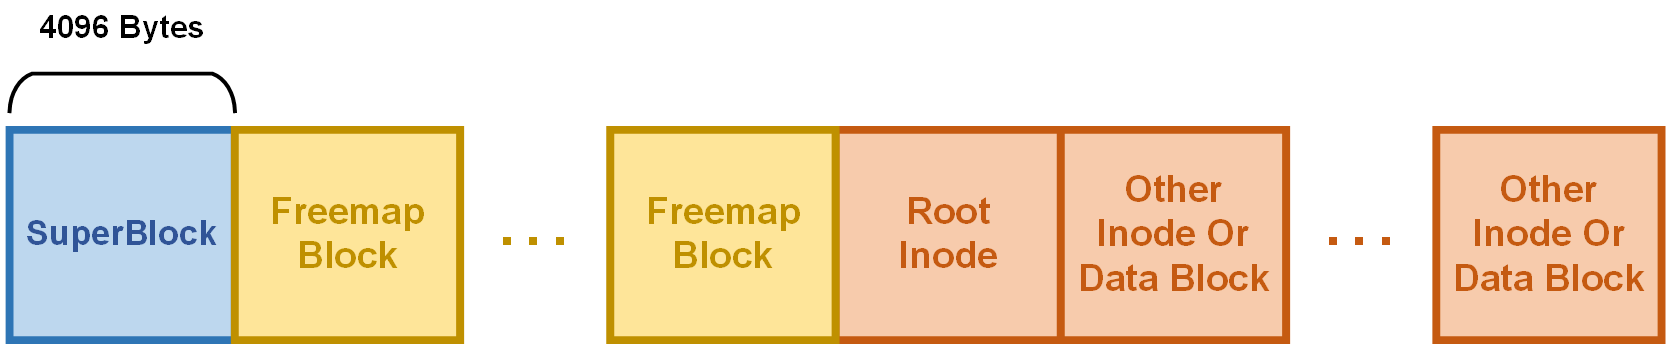
\includegraphics[width=0.85\textwidth]{sfs}
	\setlength{\abovecaptionskip}{2pt}
	\caption{SimpleFS结构}
	\label{pic:sfs}
\end{figure}

一个SimpleFS文件系统的第一块恒为超级块(SuperBlock),它记录了整个文件系统的基本信息,例如总磁盘块数、未使用的磁盘块数、Freemap块个数等。紧随其后的是若干Freemap块,它记录了整个文件系统中磁盘块的占用情况。Freemap块使用一个bit表示一个块,0为未被占用,1为已被占用。通过Freemap块Moonix就可以快速找到空闲可用的磁盘块。Freemap块后面是表示根文件系统的Inode块。SimpleFS也是以树状结构组织文件的,Root即为 “/” 文件夹。Root Inode后就是其他文件的Inode或者数据块,这些块不会做特殊的排序,查找文件需要从根目录开始查找。

\begin{lstlisting}[language={C}, caption={SimpleFS超级块结构}, label={lst:superblock}]
typedef struct {
	uint32 magic;               // 魔数
	uint32 blocks;              // 总磁盘块数
	uint32 unusedBlocks;        // 未使用的磁盘块数
	uint32 freemapBlocks;       // freemap 块数
	uint8 info[32];             // 其他信息
} SuperBlock;
\end{lstlisting}

超级块的结构如代码 \ref{lst:superblock} 所示。第一个字段就是magic number。这个字段恒为 0x4D534653,即ASCII码 “M”、“S”、“F”、“S”。Moonix初始化文件系统时,会首先检查魔数以确定文件系统类型,blocks字段表示这个文件系统一共占用多少个磁盘块。unusedBlocks字段表示这个文件系统目前剩余的空闲磁盘块个数。freemapBlocks表示Freemap块的总个数,这个字段的更重要用处在于推断出Root Inode所在的磁盘块号。最后就是info字段,这是一个字符串,记录了一些其他信息。超级块的实际内容很小,只有48字节,剩余空间由0填充。

\begin{lstlisting}[language={C}, caption={SimpleFS Inode结构}, label={lst:inode}]
typedef struct
{
	uint32 size;                // 文件大小,type 为文件夹时该字段为 0
	uint32 type;                // 文件类型
	uint8 filename[32];         // 文件名称
	uint32 blocks;              // 占据磁盘块个数
	uint32 direct[12];          // 直接磁盘块
	uint32 indirect;            // 间接磁盘块
} Inode;
\end{lstlisting}

一个 Inode 块代表了一个文件或文件夹,结构如代码 \ref{lst:inode} 所示。type字段表示该Inode所代表的文件的类型,可用取值有TYPE\_FILE(普通文件)或TYPE\_DIR(文件夹)。当type取TYPE\_DIR时,size字段为0。并且直接磁盘块和间接磁盘块都是指向存储在该文件夹下的文件的Inode。当type取TYPE\_FILE时,磁盘块指向实际的数据块。当Inode类型为文件夹时,direct[0]和direct[1]分别存储指向当前和指向上一级文件夹的 Inode。

\begin{figure}[htpb]
	\centering
	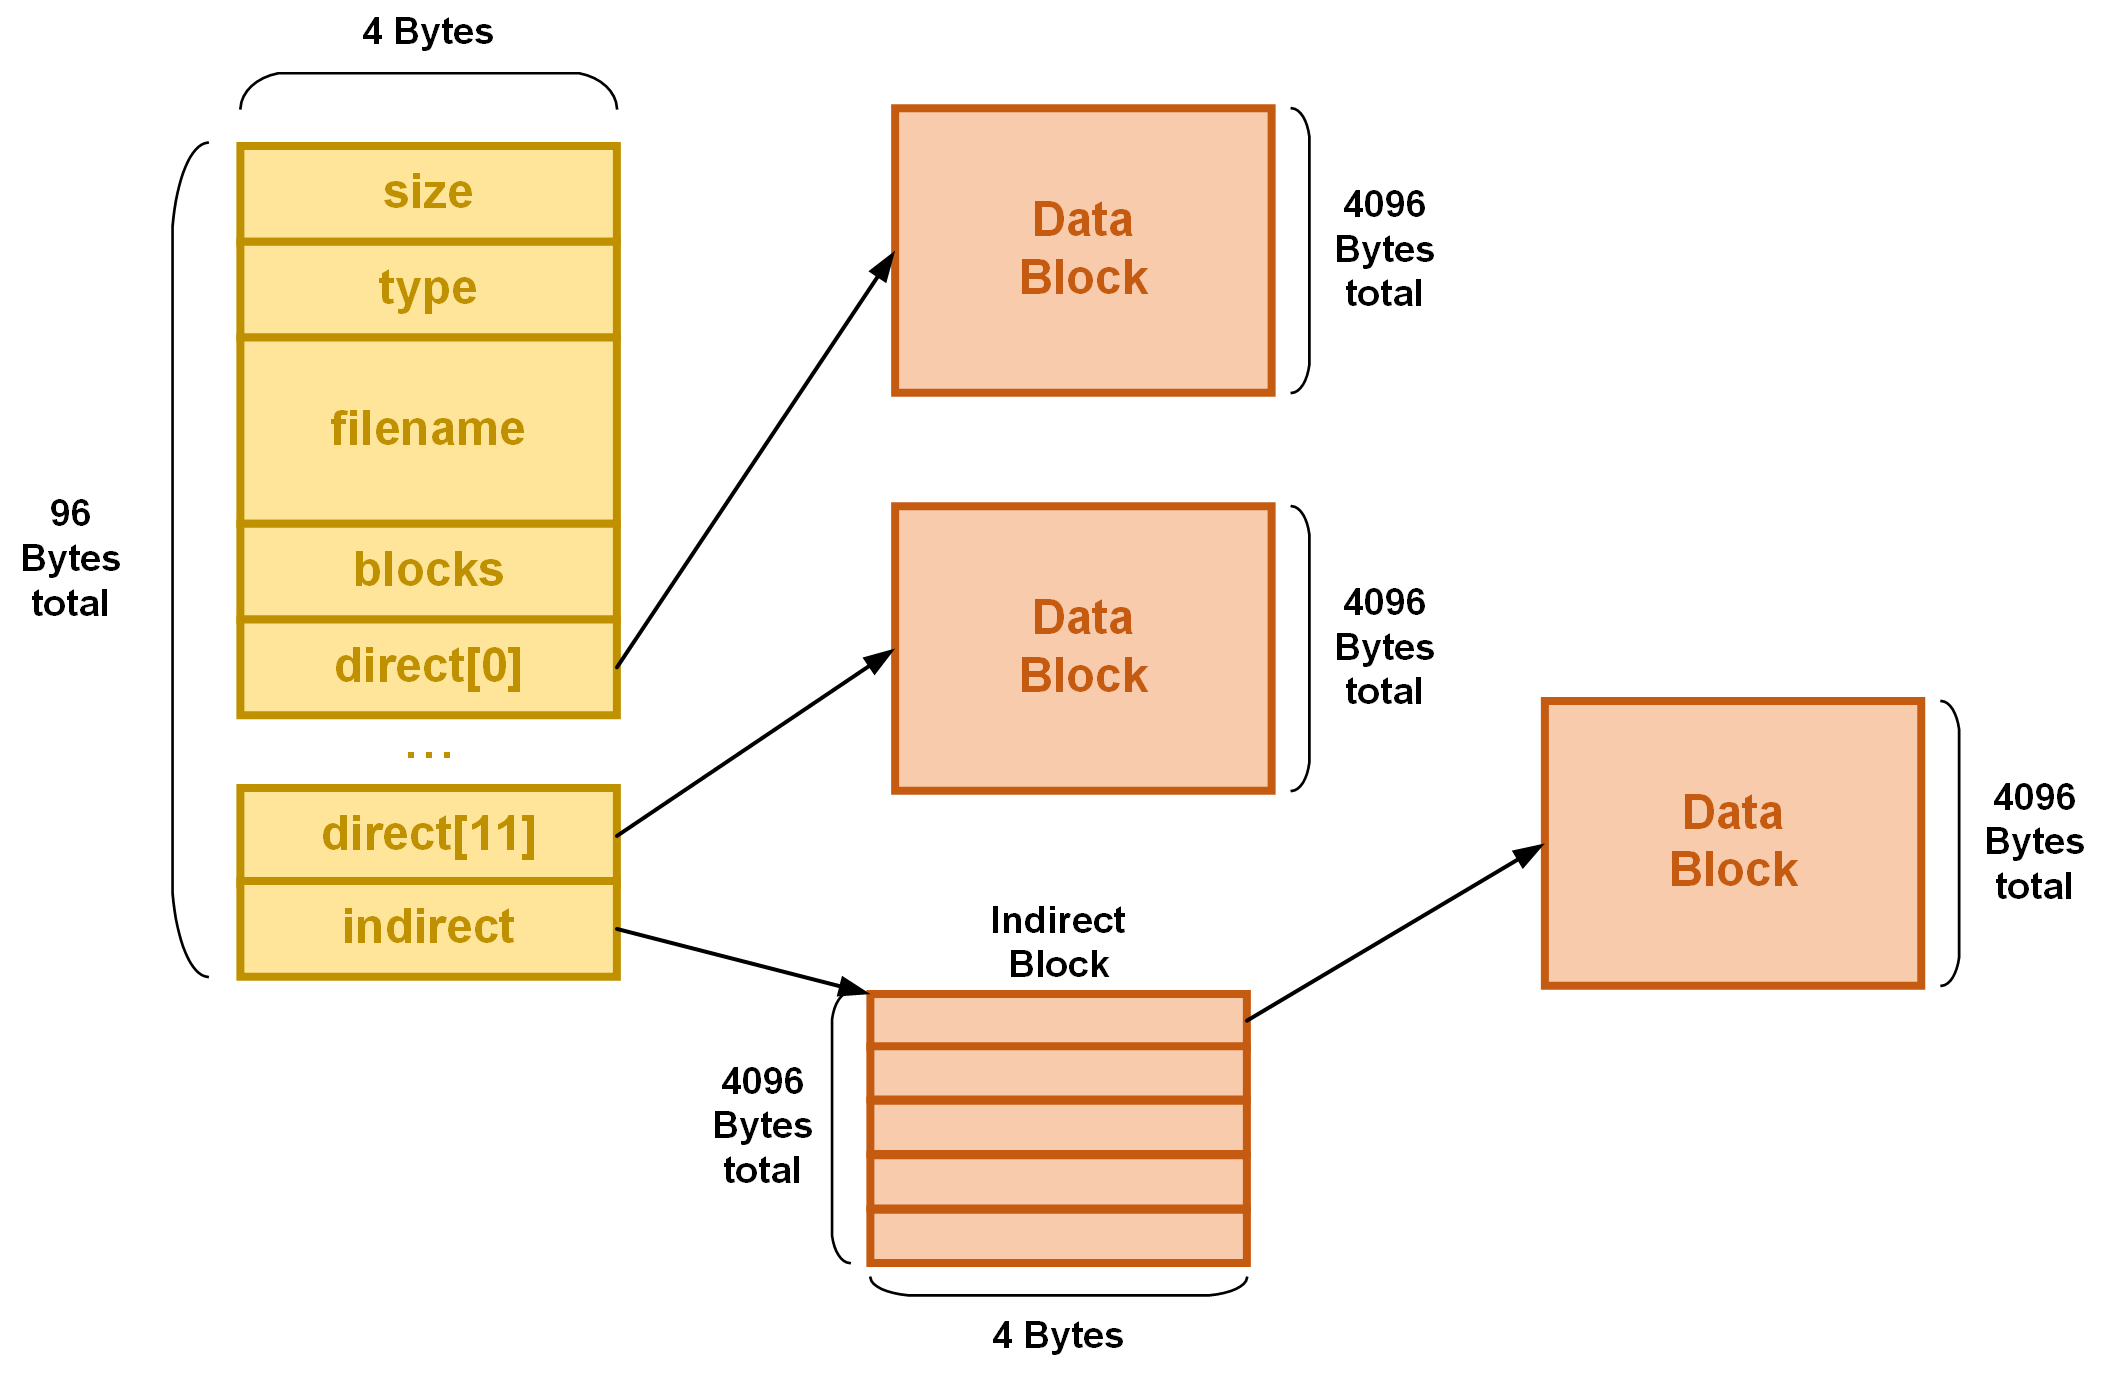
\includegraphics[width=0.70\textwidth]{inode}
	\setlength{\abovecaptionskip}{2pt}
	\caption{Inode直接磁盘块与间接磁盘块}
	\label{pic:inode}
\end{figure}

关于直接磁盘块和间接磁盘块,如图 \ref{pic:inode} 所示。每个Inode块中有一个长度为12的direct数据,如果blocks字段小于等于12,可以直接使用该数组存储磁盘块号,否则,由indirect字段指向一个Indirect Block,在该磁盘块中可以存储更多的磁盘块号。

SimpleFS 的相关数据如下:

\begin{itemize}
	\item 一个 Freemap 块可以表示 32K 个磁盘块的空闲状况
	\item 一个文件夹下,除去 “.” 和 “..” 以外,最多可以存储 1034 个文件或文件夹
	\item 单个普通文件大小最大为 4.04 MB
\end{itemize}

\section{内核驱动}

目前Moonix没有真正实现文件系统,而是在内核镜像打包时将文件系统镜像直接打包到内核的.text段中,这样Moonix系统在启动时,整个文件系统就已经存在于内存之中了,.text段中的文件系统前后都有全局符号标记,使得内核可以直接寻找到文件系统的开头。

Moonix操作系统在启动初始化时,最后一步就是去初始化文件系统,并从文件系统中获取shell可执行文件,并加载执行。文件系统的初始化工作比较简单,由于本文件系统的特性,内核只需要根据全局符号,获取到文件系统的开头字节,读入超级块解析文件系统的基本信息,寻找并缓冲root目录的Inode即可。

文件系统驱动中,lookup函数是一个比较核心的函数。lookup函数将传入的Inode作为当前目录,从当前目录下根据路径查找文件。例如,若当前目录为/usr,传入./hello和hello甚至../usr/hello都可以找到可执行文件hello。如果传入的路径以/开头,函数会忽略当前路径而从根目录下开始查找。如果传入的Inode为null,函数也会从根目录开始查找。函数会根据路径分割出需要在当前目录下查找的文件或文件夹名称,并递归调用lookup函数进一步搜索。

另一个比较核心的函数,是readall函数。readall函数传入一个文件类型的Inode。这个函数将该Inode所代表的文件数据全部拷贝到字节数组中。这个函数主要用于操作系统或者用户在执行某个可执行文件时,获取到Inode之后,需要将这个Inode所表示的文件拷贝到内核中。传入的字节数组通常是动态内存分配得到的,在操作系统解析并获取映射各个段之后,这个数组会被内核回收。